% This is an internship report my friend Gabriel wrote using tufte-style-article, and I am infinitely thankful he used the Tufte design features so nicely.
% It contains a lot of equations, graphs, pictures, chunks of code, definitions, theorems, etc. so it is really interesting to see that arranged in a Tufte way. That's why I think it is a great example of what this class can do!

\documentclass[
	a4paper,
	12pt,
	raggedright,
	twoside
]{tufte-style-article}

% SOME MORE PACKAGES AND FINE-TUNING

% Math input
\usepackage{amsthm, calrsfs}

% Even f a n c i e r tables
\usepackage{multirow}
\usepackage{colortbl}
\usepackage{hhline}

% Even better hyper refs
\usepackage{cleveref}

% Report structure
\usepackage{glossaries}

% Used for printing standard units
\usepackage{siunitx}

% Figures related packages
\usepackage{svg}
\usepackage{subfig}

\captionsetup[subfigure]{justification=centering}

\DeclareMathAlphabet{\pazocal}{OMS}{zplm}{m}{n}
\SetMathAlphabet\pazocal{bold}{OMS}{zplm}{bx}{n}

\newcommand{\hlred}[1]{\textcolor{Maroon}{#1}} % Print text in maroon
\newcommand{\ie}{\textit{i.\hairsp{}e.}\xspace} % Command to print i.e.
\newcommand{\eg}{\textit{e.\hairsp{}g.}\xspace} % Command to print e.g.
\newcommand{\todo}[1]{\textcolor{red}{TODO: #1}} % Command to print colored TODO
\newcommand{\py}[1]{\inlinecode{python}{#1}}

\theoremstyle{definition}
\newtheorem{definition}{Definition}[section]

\theoremstyle{remark}
\newtheorem*{remark}{Remark}

\makeglossaries

\newglossaryentry{VTK}{
        name=VTK,
        description={Visualization Tool Kit}
}
\newglossaryentry{AMR}{
        name=AMR,
        description={Adaptive Mesh Refinement}
}
\newglossaryentry{HTG}{
        name=HTG,
        description={Hyper Tree Grid}
}
\newglossaryentry{LOD}{
        name=LOD,
        description={Level Of Detail: The maximal depth of a given AMR tree.}
}
\newglossaryentry{FFT}{
        name=FFT,
        description={Fast Fourier Transform: Algorithm that computes the discrete Fourier transform.}
}

% Custom titlepage
\makeatletter
\renewcommand\@maketitlebis{%
    \noindent
    {\Large \itshape \@author \hfill \normalsize 19 April -- 20 August, 2021}
    \begin{minipage}{.8\textwidth}
        \vspace{4cm}
		{\huge\raggedright \@title \par }
		\vskip 20pt
		{\Large Internship report}\\
		\vskip 8pt
		Master's degree in scientific computing and modelling at the University of Rennes 1
	\end{minipage}

	\vfill
	\noindent
    \begin{tabular}{ l l  }
        \includesvg[width=1.5cm]{assets/CEA_logo_nouveau.svg} & \\
        &\\
        Receiving institution: &CEA Paris-Saclay \\
        Internship advisor: &Damien Chapon \\
        Scientific advisor: &Loïc Strafella
    \end{tabular}

    \vskip 1cm
    \noindent
    \begin{tabular}{ l l  }
        \includesvg[width=1.5cm]{assets/rennes1.svg} &\\
        &\\
        Faculty advisor: &Mariko Dunseath-Terao
    \end{tabular}

}
\renewcommand\maketitle{
    \@maketitlebis
    \thispagestyle{empty}
}
\makeatother

\title{Visualization and analysis of tree-based Adaptive Mesh Refinement simulations}
\author{Gabriel Lefloch}
\date{August, 2021}


\begin{document}

\maketitle

\cleardoublepage

\tableofcontents

\newpage

\section{Acknowledgements}
I would like to greatly thank Mr. Damien Chapon for his advice and guidance during this internship, which was essential to my global understanding of the concepts at hand. I would also like to deeply thank Mr. Loïc Strafella for his help and time, which was vital to the progress of my work. I am also grateful for the help and support of Prof. Mariko Dunseath-Terao.  I’d like to acknowledge the work and assistance of Sylvain Kern, creator of this Tufte-styled \LaTeX{} class.


\section{The CEA}
The French Alternative Energies and Atomic Energy Commission (CEA) is a research and development establishment playing a role in four main areas: defence and security; low carbon energies (nuclear and renewable energies); technological research for the industry and fundamental research in the physical sciences and life sciences.\cite{CEA} This internship took place in the Institute of Research into the Fundamental Laws of the Universe (IRFU), which is located in the Paris-Saclay center -- one of the nine in France.
To be more specific, it was held in the Laboratory of Software Engineering for Scientific Applications (LILAS). This laboratory is part of one of the seven departments of the aforementioned Institute, and is known as the DEDIP: Electronics, Detectors and Computing department. As per their website's description:\cite{DEDIP} \textit{“The main vocation of the Department of Sensor Electronics and Computer Science for Physics is to invent and build the ambitious and innovative detection instruments of the future, essential to the progress of physics studied at IRFU”}. The LILAS laboratory focuses on developing specific software tools and modules needed for the various physics experiments held in its department.
\section{Goals}
For over 10 years, the DEDIP has been developing efficient and practical tools for astrophysicists of the IRFU. These tools, such as PyMSES, are used to explore, analyse and visualize simulation outputs with complex data structures, namely tree-based \Gls{AMR} grids. In order to process these massive data outputs, the purpose-specific scientific tools need to be remarkably optimized. A recently developed data structure called \textit{vtkHyperTreeGrid} specifically made for \Gls{AMR} trees made its way in the C++ library \Gls{VTK}. Although this data format thrives on the plethora of generic \Gls{VTK} tools, it lacks specific data processing functionalities. That is why the internship will focus on the development of new efficient data processing algorithms for the vtkHyperTreeGrid format, in collaboration with the teams of the Military Applications Division (DAM) and Fundamental Research Division (DRF).

Namely, we aim at developing a particle mapping tool, 1D profiling tool and a sub-region extraction tool. Seeing as all three have been successfully implemented, we also take on the making of a volumetric data splatting tool.

In the long term, these algorithms are to be integrated into a future Python package called PyMSES 5.0. The novel package will provide useful tools for not only the astrophysicists of the IRFU, but more broadly to the entire scientific community using point-wise \Gls{AMR} grids.

\section{Introduction}
\paragraph{Preamble.}
With a growing demand to visualize and analyse large simulation data outputs, \textit{Adapative Mesh refinement } offers a trade-off between numerical accuracy, memory footprint and computational cost. This structured meshing method is efficient at tracking fine details in large regions, whilst taking up to 80\% less space in memory than other non-structured meshing strategies.\cite{HTG_dam} This report will focus on the presentation and analysis of several utilities that help exploit and process tree-based \Gls{AMR} structures.

\paragraph{Context.}
The term \textit{Adaptive Mesh Refinement} -- originally coined in 1984 by J. Berger and J. Oliger\cite{AMROriginal} -- is a method used to dynamically adapt the precision of a structured mesh in a numerical simulation whilst its solution is being calculated. \Gls{AMR} comes in response to a need for lighter meshing structures. Indeed, with the arrival of pre-exascale computing machines,\cite{tera_computer} data outputs of large-scale simulations using unstructured meshes with fully described connectivity are too cumbersome to store and visualize. In contrast, \Gls{AMR} is a trade-off between numerical accuracy, memory footprint, computational cost and can therefore improve visualization capabilities as well as resource usage.

While there are several approaches to \Gls{AMR} -- such as block-based or tree-based -- the following report will solely focus on the latter flavor. This meshing strategy, also known as point-wise \Gls{AMR}, can be found in RAMSES, a massively parallel hydrodynamical code for self-gravitating magnetized flows. It can be used in a broad set of domains, like stellar formation; proto-planetary systems; supernova explosions; interstellar medium; galactic dynamics and formation of large-scale cosmological structures to name a few.\cite{ramses} Its meshing method allows for deep spatial resolution without excessive memory overhead. However, its I/O performances were highly bottle-necked when scaled to many-core architectures: format specific binary files were used for restarts/checkpoints as well as post-processing, which led to unwieldy and heavy outputs. What's more, the data format used to describe it's meshes was proprietary and demanded purpose-specific tools.\cite{pymses_website, osiris, yt} L. Strafella and D. Chapon's recent work\cite{Strafella_2020} circumvents both dilemmas by integrating in RAMSES an efficient parallel I/O library called \textit{Hercule}, and by splitting the main data outputs into two formats: one used for checkpoints (and therefore only read by the code itself), and another for post-processing called \textit{LightAMR}. The latter format aims at giving a standard and self-descriptive way to characterize \Gls{AMR} trees, with memory efficiency in mind.

\section{The LightAMR standard} \label{sec:lightAMR}
\Gls{AMR} meshes are refined in areas of simulations that are turbulent or sensitive, so as to capture detail only where it is needed. Contrary to fixed resolution grids or meshes, this method allows for deep resolution on large-scale simulations. Tree-based \Gls{AMR} meshes are grids that are refined by subdividing their cells into sub-cells. As an example, let's consider a 2D "blast" simulation in which we follow the propagation of a mechanical wave through a bounded square space. The blast is most turbulent near the propagated wave departing the center. We should expect a higher number of cells in that region. As we can see in the figure \ref{fig:blast}, the level depth of the \Gls{AMR} grid in \ref{fig:blastLevel} matches the corresponding high density zones in \ref{fig:blastDensity}.
\begin{figure}[!htb]
    \sidecaption{\Gls{VTK} 2D rendering of the tree-based mesh of a blast simulation. The image is a snapshot at $t\approx0.06s$, with a box length of 1.0 (unitless). \label{fig:blast}}
    \subfloat[Representation of the depth or level of the grid (i.e. the subdivision level).]{
        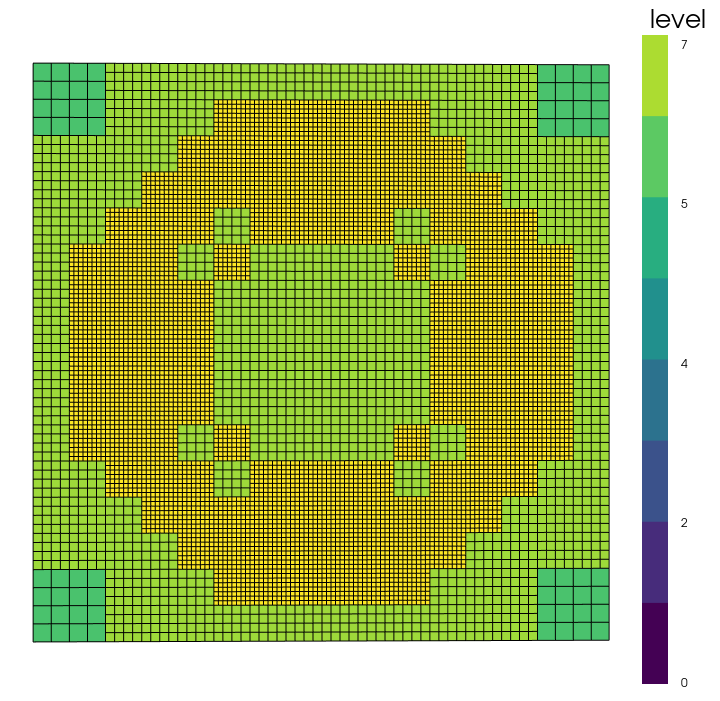
\includegraphics[width=.5\linewidth]{assets/2d_blast_level.png}
        \label{fig:blastLevel}
    }
    \subfloat[Representation of the density of the matter.]{
        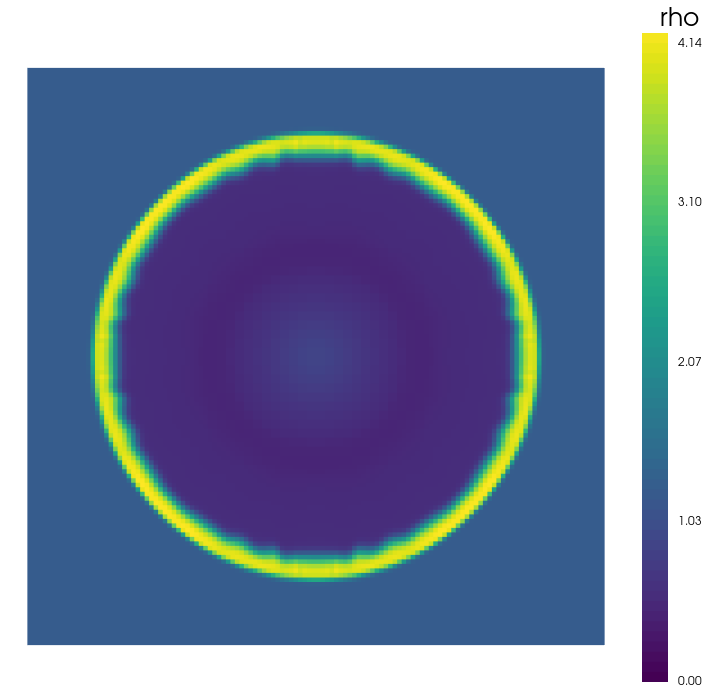
\includegraphics[width=.5\linewidth]{assets/2d_blast_density.png}
        \label{fig:blastDensity}
    }
\end{figure}
\newline
The name \textit{tree-based} \Gls{AMR} comes from the fact that each cell can be represented by a vertex of a tree. There is therefore a duality in the representation of this meshing strategy. LightAMR is a standard used to describe \Gls{AMR} trees. In fact, it is a first step towards unifying the different types of formats used to outline this meshing strategy. It is self-descriptive, in that it uses key-value pairs to give a name to each data entry. It is also memory efficient, because it fully exploits the implicit structure of tree-based grids and can be compressed for storage with an algorithm tailored to the format.\cite{compression}


Before going any further in the description of the standard, let us define a \textit{tree}:

\begin{definition}[Tree] \label{def:tree}
Given a set of vertices $V$, we define an undirected edge with the following requirements:
\begin{enumerate}
    \item[(1)] any two vertices are connected by a path,
    \item[(2)] no set of edges can form a closed polygon.
\end{enumerate}
We define the \textit{root} of our tree by one and only one element of $V$. We call \textit{leaf} a node that has no edge leaving it, and \textit{strict node} a vertex that is not a leaf. Henceforth, a tree is defined by the couple $(V, E)$, where $V$ is the set of all vertices of the tree and $E$ all its directed edges. The figure \ref{fig:treeDefinition} gives us an example of a tree.
\end{definition}
\begin{remark}
Let us note that directed edges are unambiguously deduced from the undirected ones, as any vertex of $V$ has a unique path to the root.\sidenote{Indeed, according to (1) any vertex can be connected to the root by a given path, and the axiom (2) ensures the unicity of that path (multiple paths would lead to a closed polygon)} From this, we define the \textit{depth} -- also known as \textit{level}, see figure  \ref{fig:tree_example} -- of a given vertex by the number of edges in its path from the root.
\end{remark}
\begin{figure}
    \centering
    \sidecaption{Depiction of a tree according to the definition \ref{def:tree}. Each color of a vertex matches a tree depth level. Squares delineate leaf  nodes, and circles strict nodes. The upmost vertex (in purple) is called the root. Finally, the labels are what describe the tree: 1 for parent and 0 for leaf. \label{fig:treeDefinition}}
    \includesvg[width=\linewidth]{assets/example_tree_level.svg}
\end{figure}

\begin{remark}
\begin{itemize}
    \item[]
    \item The root will always be represented at the top of the tree in this report. Thus, the tree is always a descending tree.
    \item The duality between the grid representation and the tree representation is unique, so long as we define an isomorphic mapping function between the set of vertices and the set of cells. As we'll see later on, a space filling function such as the Morton space filling curve can be used to get a unique vertex-cell pair.
\end{itemize}
\end{remark}


\paragraph{Description of a tree in LightAMR.} As we can see in the figure \ref{fig:treeDefinition}, each node label describes whether it is a leaf of a strict node. (0 being a leaf of the tree, 1 being a strict node). This is the basis behind the description of trees in the LightAMR standard. Indeed, \Gls{AMR} trees are detailed by a list or array called \texttt{isParentInt} comprised only of zeros and ones. As an example, the \texttt{isParentInt} description of the figure \ref{fig:treeDefinition} would be:
\begin{center}
    \texttt{isParentInt: 1 | 1 0 0 0 | 0 0 0 0}
\end{center}

More generally, if we define a 1 as being a strict node (that will necessarily have child nodes) and a 0 as a leaf node (indicating the end of a branch), from any \texttt{isParentInt} array we can deduce a corresponding tree representation, given two crucial parameters that are the dimension $d\in \mathbb{N^*}$ and the branching factor $f \in \mathbb{N^*}$. The number of children of each strict node is given by $f^d$.\sidenote{For the figure \ref{fig:treeDefinition}, the branching factor $f$ is 2 and the dimension is $2$. There are therefore $2^2 = 4$ children at each strict node, as is depicted.}

In addition to the \texttt{IsParentInt} array, lightAMR also comes with an array called \texttt{IsMaskInt}, which describes which vertices are to be displayed/taken into account or not. \texttt{IsMaskInt} is equally composed only of 0's and 1's -- a 1 signifies that the point is hidden or \textit{masked} while a 0 signifies the opposite. This array description will come in handy for both visualization and domain decomposition, as we'll see in forthcoming sections.

\paragraph{Domain decomposition.} In massively parallel simulation codes like RAMSES, many calculations or processes are carried out simultaneously over many physical processors so as to gain in available computation memory and lower the wall-clock time of the large simulations. In the case of tree-based \Gls{AMR} grids, carrying multiple calculation processes on a same tree can be done by separating the tree in multiple domains and then concurrently do the calculations on each domain. That can be done by partitioning the grid into multiple sub-blocks. There are multiple methods for domain decomposition of the grid among the processors, such as the famous Peano-Hilbert
space-filling curve. The figure \ref{fig:tree_domain}, based of the figure \ref{fig:tree_example} illustrates an example of a domain decomposition. In this case, there are three distinct domains.
\begin{figure}
    \centering
    \sidecaption{Domain decomposition of the previously considered tree. In this example, there are three domains indicated by the respective colors. \label{fig:tree_domain}}
    \includesvg[width=\linewidth]{assets/2d_domain_tree_example.svg}
\end{figure}

\paragraph{Checking the coherence of LightAMR.} When a tree-based \Gls{AMR} structure is saved to a file using the LightAMR format, we may add a number of additional arrays and variables so as not to have to re-compute properties of the tree every time we need them. These arrays can be for example: the number of vertices per level, the number of domains, the refinement factor $f$, the dimension $d$, the total number of cells, the total number of levels per domain, etc. The HDF5 file format can be used to store these details, as it employs a data format that stores key-value pairs of information in a hierarchical fashion.

However, as some errors can slip into the tree descriptions per domain, the coherence of the \texttt{isParentInt} and \texttt{isMaskInt} arrays has to be verified according to the other pre-computed or predefined variables. e.g: does the number of vertices per level array match the actual number of vertices in \texttt{isParentInt}? Is the \texttt{isMaskInt} coherent?\sidenote{If a vertex is marked as masked, but one of its child vertices is marked as not masked, there is a coherence problem. Indeed, if the parent vertex is masked, all the children must be aswell.} etc. These verifications are listed in the appendix as Python implementations and use HDF5 file structures.

\section{A need for a specialized tree-based AMR object: The Hyper Tree Grid}

Point-wise \Gls{AMR} grids lack widespread support in large visualization libraries, and generally\sidenote{There are visualization and analysis tools that have tree-based \Gls{AMR} grid implementations, such as the yt project.\cite{yt}} have to be converted into well known unstructured meshes in order to be visualized, which defeats the purpose of our tree-based grids. Moreover, their peculiar data-structure demands specialized tools in order to traverse and manipulate them. The DAM's recent work circumvents this dilemma by integrating tree-based data structures and tools\sidenote{Namely special constructs to traverse the trees and iso-contour filters} into the well established visualisation library \Gls{VTK} allowing for a scalable and feature rich tool-set to visualize \Gls{AMR} based simulation outputs. The object is called the \textit{HyperTreeGrid}, and was envisioned with 2 goals in mind: integrate the object into the \Gls{VTK} ecosystem in order to gain compatibility with the wealth of \Gls{VTK} tools and design high performance algorithms specific\sidenote{e.g : for the traversal of a tree, specialized constructs called cursors and supercursors were developed.} to tree-based \Gls{AMR} grids.
Let us define a Hyper Tree Grid:

\begin{definition}[Hyper Tree Grid]
In dimension $d \in \mathbb{N^*}$ with a branching factor $f \in \mathbb{N^*}$,\sidenote{In our case, $d$ and $f$ are restrained to: $d \in \{1, 2, 3\}, \ f \in \{2, 3\}$} a \Gls{HTG} object is a type of data structure that can be represented as a tree where each strict node has exactly $f^d$ children. Data can be attached to any one of its vertices.
\end{definition}

\paragraph{Visual representations.} The \Gls{HTG} object intrinsically has two visual facets: it may be represented as a tree graph or as a set of geometric shapes, as seen in the figure \ref{fig:tree_example}. Let us note that there is a trivial bijection between each node of (a) shape of (b), so long as we define the order in which the node indexes appear in (b). This order is given by the Morton space filling curve, which works in both 2D and 3D as seen in the figure \ref{fig:morton_curve}.

\begin{marginfigure}
    \includesvg[width=\linewidth]{assets/morton_curve.svg}
    \caption{This schematic reflects how the morton space filling curve is used to define the order in which nodes of a tree are represented in a 3D \Gls{HTG}. \label{fig:morton_curve}}
\end{marginfigure}

\begin{remark}
\textit{In fine,} only the level 3 of the geometric representation (b) in the figure \ref{fig:tree_example} is used to represent a \Gls{HTG} in \Gls{VTK}.
\end{remark}

\newpage
\paragraph{Implementation.} As mentioned earlier, the heart of the object is baked into a C++ scientific visualization library known as \Gls{VTK}. Any action on a \Gls{HTG} object is therefore done through the library's already existing paradigms.\sidenote[][100pt]{For instance, adding data the cells of a tree demands the usage of special \Gls{VTK} data structures such as \mintinline{C++}{vtkPointData}.} Creating a \Gls{HTG} is done by instancing it's \Gls{VTK} object, then by using a special construct called a \textit{cursor} to define and navigate the branches of our tree. In fact, \textit{cursors} (see definition \ref{def:cursor}) are a core element of the object as they are designed to fully take advantage of the implicit geometry of trees: \textit{Depth-First search} is generally used to descend the tree and, depending on the used cursor, certain pre-computations are done to have access to neighboring cell information.

\begin{definition}[Cursor]\label{def:cursor}
For a given Hyper Tree Grid $H$, a \textit{cursor} is a structure pointing to one of the vertices of $H$ used to traverse and access the nodes of its structure.
\end{definition}
While there are several cursor implementations that vary in complexity, all are equipped with two fundamental functions:
\begin{verbatim}
    ToChild(i) : move to the child of index i,
                 relative to the current vertex.
    ToParent() : go up one vertex (except if at root).
\end{verbatim}
The other implementations -- known as \textit{supercursors} -- build on top of these primitives, adding functionalities that give access to neighboring cells; the coordinates of the cell centers; bounds of the current cell; etc.

\begin{figure*}[btp]
    \centering
    \subfloat[Tree representation.]{
        \includesvg[width=.5\linewidth]{assets/htg_tree_level.svg}
        \label{fig:tree_representation}
    }
    \subfloat[Stacked levels of geometric representation.]{
        \includesvg[width=.5\linewidth]{assets/example_mesh_decomp.svg}
        \label{fig:example_mesh_decomp}
    }
    \sidecaption{Two representations of a \Gls{HTG} object with $d=2$ and $f=2$. On the left (a) is a tree graph of the object, while on the right (b) is a layered decomposition of a \Gls{VTK}-like rendering. Each color represents a level from 0 to 3. In (a), the numbers on each vertex express the global node indexes. \label{fig:tree_example}}
\end{figure*}

\paragraph{Memory storage.} Finding an efficient way to store a \Gls{HTG} object is critical, as certain simulation \Gls{AMR} outputs can be quite sizeable. Let's consider a 2D "blast" simulation in which we follow the propagation of a mechanical wave through a bounded space, depicted in the figure \ref{fig:blast}. The resulting \Gls{AMR} tree has 12629 vertices and 8 levels of depth. The memory size of the \textit{Hyper Tree Grid} \Gls{VTK} object is 47456 Bytes, while the equivalent representation of the tree with an unstructured grid object takes up 735232 Bytes: the unstructured grid object is over 15 times bigger than it's \Gls{HTG} counterpart. This difference in memory size is achieved by only storing all strict nodes and the index of their first children nodes, also called \textit{eldest nodes}.

However, the \Gls{VTK} Hyper Tree Grid Object isn't particularly well adapted to storing \Gls{AMR} meshes on the long term. Large RAMSES outputs can have tree depth of up to 16, amounting to over $\sum_{k=0}^{15} 8^k = \frac{1-8^{16}}{1-8} \approx \num{4e13}$ vertices (assuming that every branch is fully subdivided). That yields \num{160} Tera Bytes, if one cell is stored in 4 Bytes. That is a job much more well-suited for the light\Gls{AMR} standard.

\section{Particle reading and mapping}
The Hyper Tree Grid object is capable of attaching \Gls{VTK} Data structures to its leafs, such as scalar or vector fields for subsequent visualization or data processing. However, the data must first be mapped to each cell of the \Gls{HTG}: for point particles, the spatial geometry of the \Gls{HTG} and the particle coordinates have to be taken into account so as to correctly map the position of the particles to the \Gls{HTG}.

\paragraph{The particles are stored} according to the LightAMR format in HDF5 files.\cite{hdf5_docs} They are accessed through the HDF5 Python library, which gives access to the groups and attributes of a kin file with dictionary-like data structures. In our case, the particles are stored as sub-groups of domain groups, as laid out in the figure . To be more precise, they are stored as Python dictionaries, where the keys are domains and the values are dictionaries of the particle data arrays. The following code snippet outlines the data-structure of the resulting read particles.

\begin{codebox}{python}
particle_dict = {
  # Particles of domain 0
  "0": {"ids": np.array([...]), "position_x": np.array([...]), ...}
  # Particles of domain 1
  "1": ...,
  ...
}
\end{codebox}

As we can see, each domain key has a dictionary of arrays. The full list of keys is: \py{"ids"}; \py{"mass"}; \py{"position_x"}; \py{"position_y"}; \py{"position_z"}. Most are self-explanatory, except the "ids" key that is a unique identifier of each particle generated by RAMSES during the simulation.

\paragraph{Mapping the particles} requires time efficient algorithms, as the \Gls{AMR} trees can be quite sizeable. Indeed, for an \Gls{HTG} with a depth of 15 levels (typical in large simulations), there can be in a worst case scenario up to $\sum_{k=0}^{15} 8^k = \frac{1-8^{16}}{1-8} \approx \num{4e13}$ cells.


That is why we'll compare and benchmark four candidate algorithms that map particles to a tree-based \Gls{AMR} grid. The first traverses the \Gls{HTG} once only and directly finds all the particles that fit in each cell. The second uses a different strategy: for each particle, we descend the tree and find the corresponding cell, skipping the parent cells that do not contain the particle. For the last two, instead of mindlessly descending the tree testing which cell contains the particle, we directly calculate in which quadrant or octant the particle is located and descend into it. The difference between the last two is that the third is implemented with a recursive function while the fourth is iterative.

Let us note that a recursive algorithm is used in this tool to descend the tree, and is structured as laid out in the code snippet \ref{code:descent_algo}. The recursive strategy is used throughout the report in light of the way cursors are implemented; contrary to the iterative analogue, it is quite straightforward to implement a recursive descent algorithm. The iterative version would demand checking and using the \texttt{isParentInt} and \texttt{isMaskInt} lists. Furthermore, as we will see in the sections below, there are some relatively easy-to-implement optimizations to this descent method. In this recursion, the cursor descends the tree level-by-level first, and then explores the breadth of the tree, as seen in the figure \ref{fig:2d_tree_descent}.

\begin{marginfigure}
    \centering
    \includesvg[inkscapelatex=false, width=\linewidth]{assets/2d_tree_descent.svg}
    \caption{Order in which the nodes are met by the cursor. \label{fig:2d_tree_descent}}

\end{marginfigure}

\begin{snippetnum}{python}{General algorithm used to fully descend and explore an \Gls{AMR} tree. The cursor descends the tree down to the level defined by \texttt{maxLOD}, which stands for maximum level of detail.}{code:descent_algo}
def descendTreeRec(cursor, maxLOD):
    if( cursor.GetLevel() >= maxLOD ):
        return

    if( cursor.IsLeaf() ):
        return
    else:
        for ison in range(cursor.GetNumberOfChildren()):
            cursor.ToChild(ison)
            descendTreeRec(cursor, maxLOD)
            cursor.ToParent()
\end{snippetnum}

\paragraph{Two main benchmarking tests} will be led.
For the first, we fix the dimension $d$, raffinement factor $f$ and maximal depth of the tree \texttt{maxLevel}. Then we evaluate the mapping time of each algorithm in $n = 10$ points, where each point is a set of randomly generated particles. The sets range in cardinality from \texttt{minN} to \texttt{maxN}. We are therefore evaluating the mapping time as a function of the number of particles to map.
For the second, we fix the dimension $d$, raffinement factor $f$ and the particle dataset that will be mapped with a cardinality of $p\in \mathbb{N^*}$. Then we retain the mapping time of the particle dataset over 10 different random \Gls{AMR} trees of increasing depths (ranging from \texttt{minDepth} to \texttt{maxDepth}. Thus, we evaluate the mapping time as a function of the depth of the tree.


Both benchmark results can be found in the figures \labelcref{fig:particle_mapping_n,fig:depth_mapping}. For the first test, all the curves seem to scale linearly. The third and fourth algorithms outmatch the two first in the three dimensional case. However, in 2D the first algorithm bests all the others.

For the second test, the curves are clearly no longer linear. The first algorithm is most notable, as it seems to follow an exponential growth in both dimensions. This can be an obvious pre-indicator that it does not scale well over large \Gls{AMR} tree structures. While the second algorithm fares the worst in 2D, is still leads ahead of the first in 3D. In both dimensions, the algorithms three and four lay unsurpassed.

\begin{figure}[h!]
    \centering
    \sidecaption{Mapping time of randomly generated particles ranging in numbers from 10 to 100000 using a random \Gls{AMR} tree with a maximal depth of 10. ( \texttt{maxLevel} = 10, \texttt{minN}=100000, \texttt{maxN}=1000000, $f=2, n =10$, ). \label{fig:particle_mapping_n}}
    \subfloat[2D tree, $d=2$.]{
        \includesvg[pretex=\small,inkscapelatex=false, keepaspectratio, width=\linewidth]{assets/increasingTreeDepth2D.svg}
        \label{fig:n_2D}
    }

    \subfloat[3D tree, $d=3$.]{
        \includesvg[pretex=\small,inkscapelatex=false, keepaspectratio, width=\linewidth]{assets/increasingTreeDepth3D.svg}
        \label{fig:n_3D}
    }
\end{figure}

\begin{figure}[h!]
    \centering
    \sidecaption{Mapping time of a generated particle dataset onto 10 random \Gls{AMR} trees ranging in depth from 3 to 14. (\texttt{minDepth}=3, \texttt{maxDepth}=14, $f=2, n =10, p=10000$). \label{fig:depth_mapping}}
    \subfloat[2D tree, $d=2$.]{
        \includesvg[pretex=\small,inkscapelatex=false, keepaspectratio, width=\linewidth]{assets/increasingParticleNumber2D.svg}
        \label{fig:depth_2D}
    }

    \subfloat[3D tree, $d=3$.]{
        \includesvg[pretex=\small,inkscapelatex=false, keepaspectratio, width=\linewidth]{assets/increasingParticleNumber3D.svg}
        \label{fig:depth_3D}
    }
\end{figure}

\paragraph{Results analysis.} Both benchmark reveal that the first algorithm can be used as a mapping strategy in 2D, so long as the tree is not exceedingly deep. Indeed, the figure \Cref{fig:depth_mapping} proves that the algorithm scales terribly in deep (depth=13+) trees, no matter the dimension. This is to be expected, as the first algorithm uses a binary search algorithm to filter out all the particles that fit in the $x$ bounds of a cell. From the found $x$-matching particles, we select the ones that match the $y$ bounds and then $z$ bounds if in 3D. The extra evaluation done in 3D dramatically lowers the overall performance.

\begin{marginfigure}
    \centering
    \includesvg[width=\linewidth]{assets/alg4.svg}
    \caption{Schematic of a 2D cell subdivided into 4 subcells, ordered by the z-curve illustrated in figure \ref{fig:morton_curve}. The black dot represents a particle $P$, with $(x,y)$ as it's coordinates. \label{fig:alg4}}
\end{marginfigure}

The better performance scaling of the algorithms 2,3,4 observed in the figures \ref{fig:depth_2D},\ref{fig:depth_3D} is directly linked to the \textit{cursors} used to navigate the tree. These constructs are extremely lightweight and fully exploit the tree nature of point-wise \Gls{AMR} grids for moving from vertex to vertex.
In all the other cases, the algorithms 3 and 4 are quite comparable and seem to always outmatch the others. This can be explained by the fact that the descent to the correct cell is done automatically and optimally. There is no search, contrary to the algorithms 1 and 2. The figure \ref{fig:alg4} will help us illustrate the algorithm: to find in which quadrant the particle lies, we simply have to evaluate the following conditions:
\begin{align}
x \in \left [ x_{min}; \frac{x_{min}+x_{max}}{2} \right ],
y \in \left [ y_{min}; \frac{y_{min}+y_{max}}{2} \right ]
\implies \text{P in quadrant 1}
\end{align}

\begin{align}\label{eq:quadrant}
x \in \left [ \frac{x_{min}+x_{max}}{2}; x_{max} \right ],
y \in \left [ y_{min}; \frac{y_{min}+y_{max}}{2} \right ]
\implies \text{P in quadrant 2}
\end{align}

\begin{align}
x \in \left [ x_{min}; \frac{x_{min}+x_{max}}{2} \right ],
y \in \left [ \frac{y_{min}+y_{max}}{2}; y_{max} \right ]
\implies \text{P in quadrant 3}
\end{align}

\begin{align}
x \in \left [ \frac{x_{min}+x_{max}}{2}; x_{max} \right ],
y \in \left [ \frac{y_{min}+y_{max}}{2}; y_{max} \right ]
\implies \text{P in quadrant 4}
\end{align}
In the example given in the margin figure \ref{fig:alg4}, it is the equation \ref{eq:quadrant} that holds true. By iteratively (or recursively) applying this strategy, we directly find the leaf of the tree containing $P$.

Finally, we may ask ourselves whether it is best to use an iterative or recursive algorithm. By singling out both the algorithm 3 and 4 (figure \ref{fig:difference}) of figure \ref{fig:depth_3D}, we notice that the recursive flavor of the two is marginally faster. However, choosing between the two is of little importance: both perform virtually the same, and recursion is very language specific. What's more, recursion may be easier to read in well suited cases but may also use more memory than iteration.

\begin{figure}
    \centering
    \sidecaption{A plot of \ref{fig:depth_3D}, but only with the algorithms 3 and 4. \label{fig:difference} }
    \includesvg[pretex=\small,inkscapelatex=false, keepaspectratio, width=\linewidth]{assets/only34.svg}
\end{figure}

To recap, we can look at the average times for both benchmark tests per dimension (figure \ref{fig:mappingAvg}). It is clear that either the methods 3 or 4 should be used. The first can be used in the specific case of 2D trees.

\begin{figure}[h!]
    \centering
    \sidecaption{Average mapping times of both benchmarks per dimension. \label{fig:mappingAvg}}
    \includesvg[pretex=\small,inkscapelatex=false, keepaspectratio, width=.5\linewidth]{assets/mappingAverages.svg}
\end{figure}

\FloatBarrier

\begin{remark}
The trees used for the benchmarks are randomly generated. The code used to generate them can be found in the appendix \ref{code:AMR_generator}.
\end{remark}

\section{Extraction of a \Gls{HTG} sub-region}
\begin{marginfigure}
    \includesvg[width=\linewidth]{assets/cube_dim.svg}
    \caption{Illustration of the two coordinate systems of origins $O$ and $O'$, with $\pazocal{H}$ represented in $O$ and $R$ in $O'$. \label{fig:cube_dim}}
\end{marginfigure}

Certain post-processing tools do not always require the entire \Gls{HTG} but only a sub-region of it. This is the case when we want to map particles to a smaller given region so as to lower calculation times, or analyse fields of a small part of the \Gls{HTG} and not the entire domain, etc. That is why we may try to implement a function that extracts and returns a sub-domain of a given Hyper Tree Grid object with a given Level-Of-Detail (\Gls{LOD}).


\paragraph{Method construction.} Let us consider two Cartesian coordinate systems of origins $O$ and $O'$. Both are are defined by the basis vectors $\vb{(u_x, u_y, u_z)}$. Let $\pazocal{H}$ be a unitary cubic \Gls{HTG} object, centered to the origin $O$. We then define a region $R$ as the set of all triplets $(x, y, z) \in \mathbb{R}^3$ meeting the condition $C(x, y, z)$ in the second coordinate system of origin $O'$  . i.e:
\[
R = \{ \forall (x, y, z) \in \mathbb{R}^3 \ \ | \ \ C(x,y,z) \ \ \text{holds true} \}
\]

The figure \ref{fig:cube_dim} gives an example representation of the two coordinate systems in $O$ and $O'$. A cell of $\pazocal{H}$ can be considered in $R$ if it's center point coordinates are in $R$ (see illustration \ref{fig:extract_cuboid}). As a initial solution, we could descend in every cell of the tree down to a certain \Gls{LOD} and simply check if the cell center point is contained in $R$. However, the center point $(P_{\text{ center}})_{O} = (x_P, y_P, z_P)$ of a cell of $\pazocal{H}$ is expressed in the $(O,\vb{u_x, u_y, u_z})$ coordinate system and needs to first be expressed in $(O',\vb{u_x, u_y, u_z})$, where $O' = (x_{O'}, y_{O'}, z_{O'})$ :
\[
    (P_{\text{ center}})_{O'} = (x_{P'}, y_{P'}, z_{P'}) = (x_P- x_{O'}, y_P- y_{O'}, z_P- z_{O'} )
\]

In this report, only cuboidal and spherical regions are implemented. However, other types of regions can easily be implemented into the \py{Region} class. For a spherical region $R_{\text{sphere}}$, $C_r$ may be defined as follows:
\begin{equation}\label{eq:spherical_region}
C_r(x,y,z)=\begin{cases}
          1 \quad &\text{if} \, x^2 + y^2 + z^2 \leq r \\
          0 \quad &\text{otherwise} \\
     \end{cases}
\end{equation}
\noindent
where $r$ is the radius of $R_{\text{sphere}}$. For a cuboidal region $R_{\text{cube}}$, the condition function $C_{w, h, l}$ takes three parameters $(w, h, l)\in\R_+$ which are respectively the lengths along the x-axis, y-axis and z-axis of the cuboid. $C_{w, h, l}$ is defined as such:
\begin{equation}\label{eq:cuboidal_region}
C_{w, h, l}(x,y,z) =  \left\{
    \begin{array}{llccc}
        1 \quad &\text{if} \, & x_{O'} -- \frac{1}{2}w &\leq x &\leq x_{O'} + \frac{1}{2}w, \\
                &             & y_{O'} -- \frac{1}{2}h &\leq y &\leq y_{O'} + \frac{1}{2}h,\\
                &             & z_{O'} -- \frac{1}{2}l &\leq z &\leq l_{O'} + \frac{1}{2}l \\
        0 \quad &\text{otherwise} &\\
    \end{array}
    \right.
\end{equation}

\begin{figure}
    \centering
    \sidecaption{2D Illustration of the conditions used to determine if a cell in a given region $R$. Each cell center is depicted by a dot. The blue dots are the cell centers inside the region $R$. This concept is trivially extended to 3D space. \label{fig:extract_cuboid}}
    \includesvg[width=.6\linewidth]{assets/extract_cuboid.svg}
\end{figure}

\paragraph{Implementation.} The extraction tool is to be implemented in python. It can be envisioned as a class \py{HyperTreeGridExtractor} that inherits from a parent class \py{Region} which defines regions and a method for finding if a point is in the region, as depicted in the figure \ref{fig:extract_inheritance}. Such a class structure allows for a modular approach to how the regions are defined and checked, because there is no modification needed in the \py{HyperTreeGridExtractor} class. Regions can be added and checked in the \py{Region} class, according to the users' needs. The code extract \ref{code:region_class} is a minimal structure of the fully implemented \py{Region} class. At its instantiation, it initialises the center and bounds of the domain $R$, as well as a class method name \py{regionCheckFunction} used to check the \Gls{HTG}. A generic method \py{self.isInRegion()} is assigned to \py{regionCheckFunction} and can be used without further specification of the region in the subclass \py{HyperTreeGridExtractor}. The code extract \ref{code:HTG_extract_class} is also a barebone structure of the full implementation. On instantiation, its parent class is initialized and the \py{self.extract()} method can be called. The \py{extract} method invokes a recursive function \py{self._recursive_extraction()} that navigates the flagging\sidenote{Cells are flagged by specifying if they are masked or not. A masked cell is designated by a $0$ in \texttt{isMaskInt} } which cells are in the aforementioned region and which aren't.

Once we have updated the \texttt{isMaskInt} list by flagging the cells that aren't in $R$, we use a method designed to prune the branches that are masked. This reduces the original \Gls{HTG} $\pazocal{H}$ to a new smaller one $\pazocal{H'}$ that is encapsulated by the region $R$.

\begin{figure}[h!]
    \centering
    \sidecaption[][-25pt]{Class inheritance and structure of the extractor tool. \label{fig:extract_inheritance}}
    \includesvg[width=\linewidth]{assets/extract_inheritance.svg}
\end{figure}

\begin{snippetnum}{python}{Main structure of \texttt{Region} class. Region parameters are passed in the \texttt{\_\_init\_\_} function, so as to define it's center, bounds and check function used to validate if a cell is in the region in a generic fashion.}{code:region_class}
class Region(object):
  _cellCenter = [0]*3

  def __init__(self, center, regionBounds, regionCheckFunction):
    # Center of region
    self._center = np.array(center)
    # Array like defining the bounds
    self._regionBounds = regionBounds
    # Define the generic method isInRegion()
    # used to check if cell is in region
    try:
      self.isInRegion = eval("self."+regionCheckFunction)
    except:
      print("regionCheckFunction method is not defined in Region Class")

  # The following methods are the available names for regionCheckFunction
  def isInSphericalRegion(self):
    # Code to check if _cellCenter is in region
    pass
    return True

  def isInCuboidalRegion(self):
    # Code to check if _cellCenter is in region
    pass
    return True

  # Other region functions

\end{snippetnum}


\begin{snippetnum}{python}{Main structure of \texttt{HyperTreeGridExtractor} class. As we can see, checking if a cell is in the region remains completely generic. }{code:HTG_extract_class}
class HyperTreeGridExtractor(Region):

  def __init__(self, center, regionBounds, regionCheckFunction):
    # Initilaize the region parent class
    super().__init__(center, regionBounds, regionCheckFunction)

  def extract(self, HTG):
    # Define a cursor
    cursor = HTG.NewNonOrientedGeometryCursor(0, True)
    # Recursively go through the tree
    self._recursive_extraction(cursor)
    # Remove the cells that are flagged as not in the region
    clean_HTG = self.__magic_squeeze2(HTG)

    return clean_HTG

  def _recursive_extraction(self, cursor):
    cursor.GetPoint(self._cellCenter)

    # Use generic method defined in parent class
    if( (not self.isInRegion()) and cursor.IsLeaf() ):
      # Flag leafs to be removed
      cursor.SetMask(True)
      return

    if( not cursor.IsLeaf() ):
      for ison in range(0, cursor.GetNumberOfChildren()):
        cursor.ToChild(ison)
        self._recursive_extraction(cursor)
        cursor.ToParent()

\end{snippetnum}

Let's examine an example in which we define a cuboidal region $R$ with side lengths equal to 1,\sidenote{$(w,h,l)=(1,1,1)$} centered in $O' = (1, 1, 1)$. We take a cubic Hyper Tree Grid $\pazocal{H}$ made from a blast simulation with side lengths of 2 and center $O = (0, 0, 0)$. This region therefore extracts the $(1,1,1)$ corner octant of  $\pazocal{H}$. The figure \ref{fig:extraction} is the output result of the code given in \ref{code:HTG_extract_class}. As we can see, the mapped scalar density field in \ref{fig:cube_original} has been retained \ref{fig:cube_extracted}.

\begin{figure}[h!]
    \centering
    \sidecaption{
    Example of an extracted region of a given Hyper Tree Grid Object $\pazocal{H}$, made from a blast simulation. On the left (a) is the original, with a scalar density field mapped to its cells. On the right (b) is an extracted region $R$ of $\pazocal{H}$, where $R = \{(x,y,z) \in \mathbb{R}^3 \ \ | 0.5 < x, y, z < 1 \}$ . \label{fig:extraction}}
    \subfloat[Original \Gls{HTG} $\pazocal{H}$.]{
        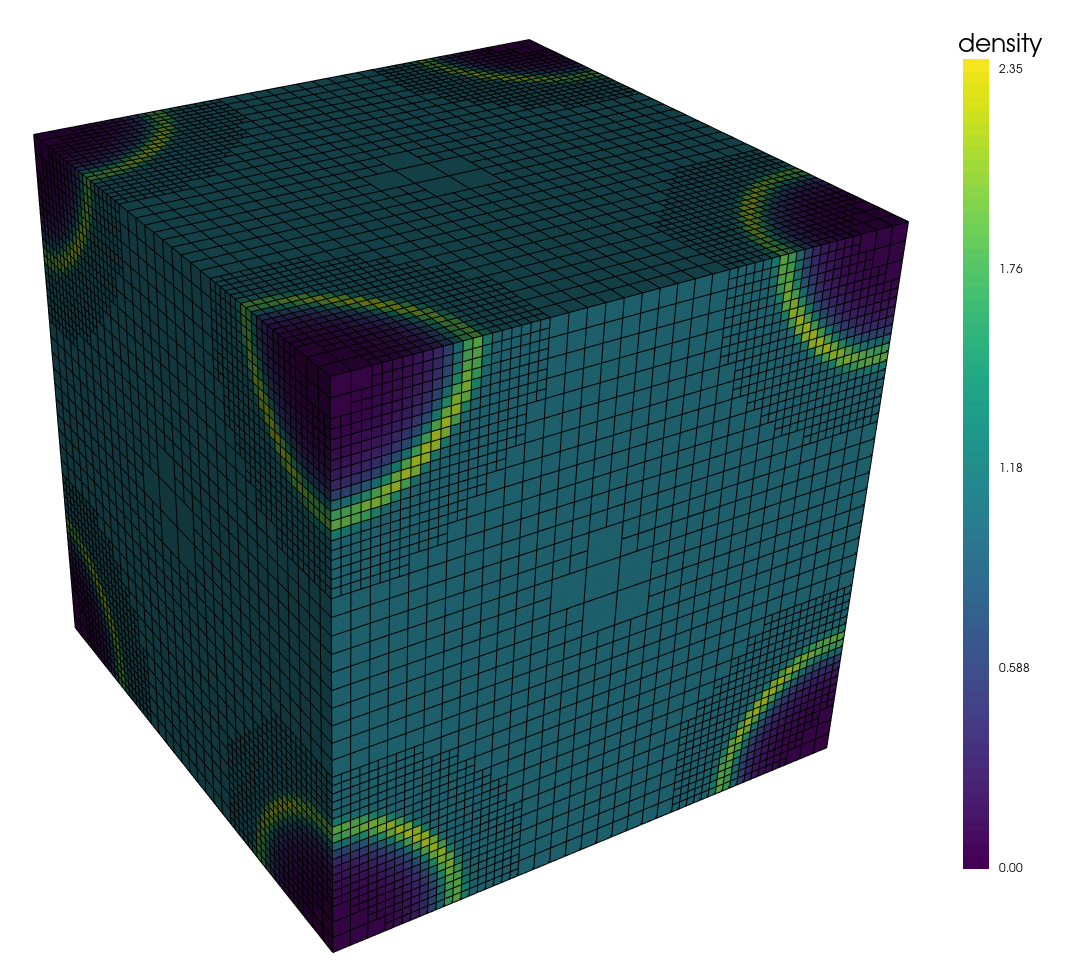
\includegraphics[width=.48\linewidth]{assets/cube_original.png}
        \label{fig:cube_original}
    }
    \subfloat[Extracted \Gls{HTG} $\pazocal{H'}$.]{
        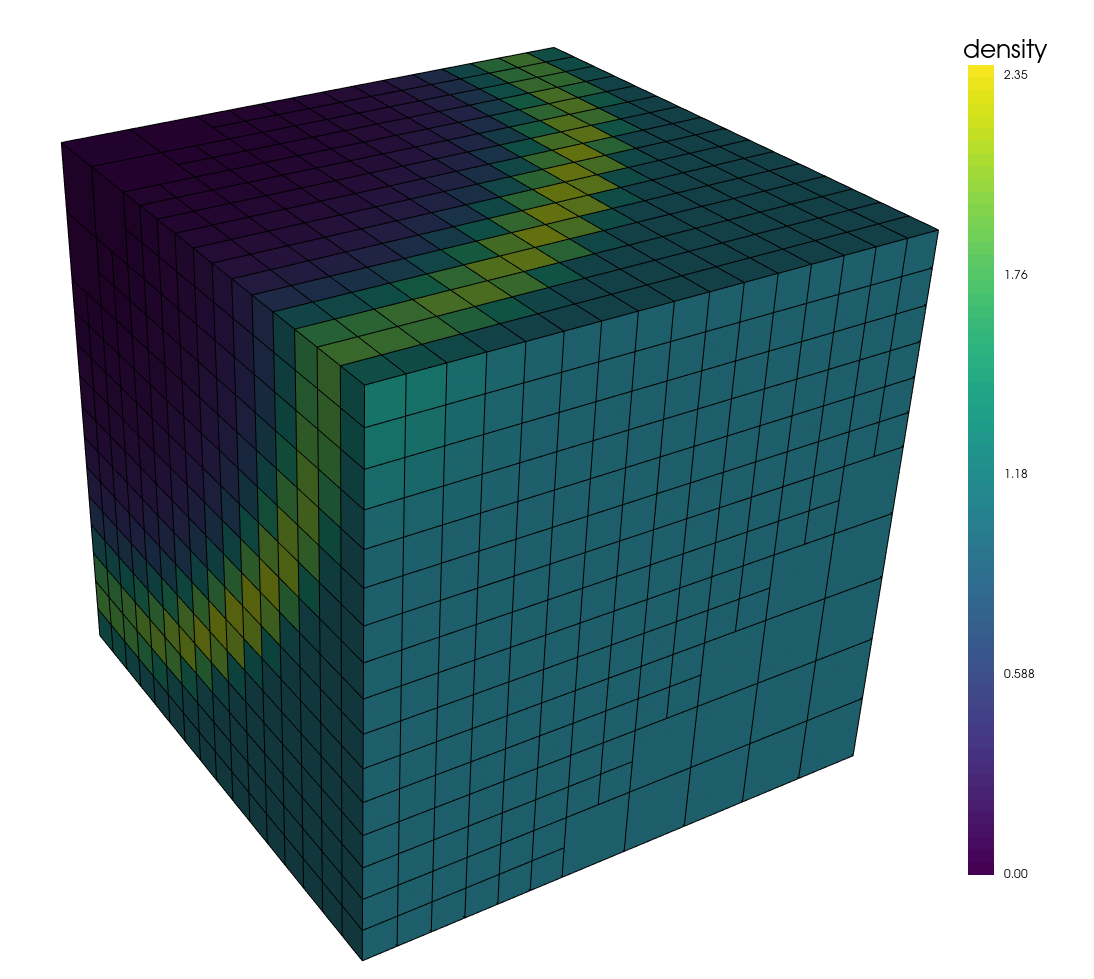
\includegraphics[width=.48\linewidth]{assets/cube_extracted.png}
        \label{fig:cube_extracted}
    }
\end{figure}

\paragraph{Performance.} It may be interesting to see how well the tool scales when extracting regions with increasing levels of depths, for a given \Gls{HTG} object. That is why we shall perform 12 extractions of two regions $R_\text{sphere}$ and $R_\text{cuboid}$ on the aforementioned blast simulation found in \ref{fig:extract_cuboid}. Each extraction will be done with an increasing \Gls{LOD} ranging from 4 to 15, the maximal level of the simulation output. The resulting benchmarks are plotted in the figure \ref{fig:extraction_perf}. Unsurprisingly, the extraction times of both regions seem to have the same global variation trends, with the cuboidal region fairing overall less well than the spherical region. There are however more operations done for the cuboidal region than its spherical equivalent, as seen in the equations \ref{eq:spherical_region} and \ref{eq:cuboidal_region}. To be more specific, $C_r(x,y,z)$ in \ref{eq:spherical_region} accounts for $\approx$ 7 operations while  $C_{w, h, l}$ accounts for $6*3=18$ operations.

As for the scaling over tree depth levels of the region extraction tool, the results in the figure \ref{fig:extraction_perf} are not very indicative of how well the tool performs. However, by plotting the region extraction times as a function of the descent times of a cursor descending the tree to each \Gls{LOD} (see \ref{fig:extraction_scaling}, we notice a roughly linear relationship between the two. This proves that the tool will scale approximately as well as the highly optimized Hyper Tree Grid cursor object, or at least as well as the function \py{isInRegion()} which is what degrades the linear relationship found in \ref{fig:extraction_scaling}. A poorly optimized \py{isInRegion()} function may therefore greatly hinder the extraction performances.

\begin{figure}[h!]
    \centering
    \sidecaption{Extraction times of both regions as a function of \Gls{AMR} tree depth levels ranging from 4 to 15. \label{fig:extraction_perf}}
    \includesvg[pretex=\small,inkscapelatex=false, keepaspectratio,width=\linewidth]{assets/extractionTimeRegions.svg}
\end{figure}
\begin{figure}[h!]
    \centering
    \sidecaption{Extraction times of both regions as a function of the descent times of a cursor in the same tree. The descent and extraction times are done over levels ranging from 4 to 15. \label{fig:extraction_scaling}}
    \includesvg[pretex=\small,inkscapelatex=false, keepaspectratio,width=\linewidth]{assets/descentTimeByExtraction.svg}
\end{figure}

\section{Extraction of a 1D profile of a scalar field}\label{sec:1d_profile}
When displaying a 3D hyper Tree Grid object through \Gls{VTK}, only the outermost surface and its attached data fields can be represented. Yet, visualizing the internals of \Gls{HTG}s is a crucial element in the scientific analysis of simulation outputs. That is why we will examine two main approaches to the problem: both involve representing the intersection of a \Gls{HTG} object with either a 1D curve or a 2D surface. Seeing as the latter approach has already been tackled and integrated into \Gls{VTK}, \cite{HTG_dam} we will focus on the 1D intersection tool. The main goal of this tool is to extract the intersection between the cells of a \Gls{HTG} $\pazocal{H}$ and a line segment $S$ in space. Once the cells are extracted, one can plot the values attached to them as a function of the length of the segment.
This section will be based of an efficient Ray-box intersection algorithm.\cite{ray_casting} We start by working in a 2D space for visualization purposes, then generalize to three dimensions.
\paragraph{Method construction.} Let $S$ be a segment in a Cartesian coordinate system of origins $O$. $S$ is defined by two points $P_a = (x_a, y_a)$ and $P_b = (x_b, y_b)$. Let's now consider the parametric equations that defines $S$:
\begin{align}\label{eq:parametric}
\begin{cases}
x(t) &= x_a + (x_b -- x_a)t \\
y(t) &= y_a + (y_b -- y_a)t
\end{cases}
\hspace{5pt} t \in [0, 1]
\end{align}
From the equation \ref{eq:parametric}, we solve for $t$ and deduce the following:
\begin{equation}\label{eq:para_eq}
    \frac{x-x_a}{x_b -- x_a} = \frac{y-y_a}{y_b -- y_a}
\end{equation}

\begin{marginfigure}
    \centering
    \includesvg[width=\linewidth]{assets/cell_intersect.svg}
    \caption{Illustration of 2D cell geometry. \label{fig:cell_intersect}}
\end{marginfigure}

Let $C$ be a square cell defined by two points $C_{min} = (x_{min, cell}, y_{min, cell})$ and $C_{max} = (x_{max, cell}, y_{max, cell})$, as is shown in the illustration \ref{fig:cell_intersect}. $S$ intersects the sides of $C$ if the following equations hold true:

\begin{align}
\begin{cases}
    x_{min} &\leq x \leq x_{max} \\
    y_{min} &\leq y \leq y_{max}
\end{cases}
\\
\implies
\begin{cases}\label{eq:bound_cond}
    \frac{x_{min, cell} -- x_a}{x_b -- x_a} &\leq \frac{x -- x_a}{x_b -- x_a} \leq \frac{x_{max, cell} -- x_a}{x_b -- x_a} \\
    \frac{y_{min, cell} -- y_a}{y_b -- y_a} &\leq \frac{y -- y_a}{y_b -- y_a} \leq \frac{y_{max, cell} -- y_a}{y_b -- y_a}
\end{cases}
\end{align}

When combining the equations \ref{eq:bound_cond} and \ref{eq:para_eq}, new minimal boundary intersection requirements can be derived.
Consider $x = x_{min, cell}$, which gives

\begin{align}
\frac{x_{min, cell} -- x_a}{x_b -- x_a} &\leq \frac{x_{min, cell} -- x_a}{x_b -- x_a} \leq \frac{x_{max, cell} -- x_a}{x_b -- x_a}
\\
\ref{eq:bound_cond} \text{ and } \ref{eq:para_eq} \implies
\frac{y_{min, cell} -- y_a}{y_b -- y_a} &\leq \frac{x_{min, cell} -- x_a}{x_b -- x_a} \leq \frac{y_{max, cell} -- y_a}{y_b -- y_a}
\end{align}
Therefore, $S$ is out of the $x$-axis range $[x_{min}, x_{max}]$ of $C$ if
\[
\frac{y_{max, cell} -- y_a}{y_b -- y_a} < \frac{x_{min, cell} -- x_a}{x_b -- x_a}
\]
If we note
\begin{align}
    t_{x,min} &= \frac{x_{min, cell} -- x_a}{x_b -- x_a} \\
    t_{y,min} &= \frac{y_{min, cell} -- y_a}{y_b -- y_a} \\
    t_{x,max} &= \frac{x_{max, cell} -- x_a}{x_b -- x_a} \\
    t_{y,max} &= \frac{y_{max, cell} -- y_a}{y_b -- y_a}\
\end{align}
then we directly deduce the two following boundary conditions that reveal if $S$ intersects $C$ or not:
\begin{enumerate}
    \item $t_{y,max} < t_{x,min}$
    \item $t_{x,max} < t_{y,min}$
\end{enumerate}
The conditions are trivially extended to three dimensions by defining two extra variables $t_{min}$ and $t_{max}$ such that
\begin{gather}
    t_{min} = \max ( t_{x,min} , t_{y,min} ) \\
    t_{max} = \min ( t_{x,max} , t_{y,max} )
\end{gather}
These two variables inform us on the minimal bounding box of $S$. In 3D, we can now add the final boundary condition:
\begin{enumerate}
    \item[3.] $t_{z,max} < t_{min}$
    \item[4.] $t_{max} < t_{z,min}$
\end{enumerate}
By once again calculating $ t_{min} = \max ( t_{z,min} , t_{min} )$  and $t_{max} = \min ( t_{z,max} , t_{max} )$, we can at last verify if the limits of our segment $S$ have not been exceeded. i.e:
\begin{equation}\label{eq:min_bounds}
    0 \leq t_{min} \leq t_{max} \leq 1
\end{equation}
If \ref{eq:min_bounds} is not true, the cell is not in the minimal bounding box of $S$. The figure \ref{fig:min_bounding} gives an illustration of the minimal bounding of a segment $S$.
\begin{figure}
    \centering
    \sidecaption{Illustration of the minimal bounding box of a segment $S$ in 2D. The colored cells are the ones intersected by the segment. \label{fig:min_bounding}}
    \includesvg[width=.6\linewidth]{assets/intersection.svg}
\end{figure}

\paragraph{Implementation.} The tool is implemented in Python as a class that takes 2 parameters to be initialized: \py{HTG}, \py{field}.\sidenote{Two others are optional \py{maxLevel=99}, \py{intersectionField=None}. \py{maxLevel} specifies the maximum tree depth level used when traversing the tree. py{intersectionField} is the name of a scalar field  that is attached to the \py{HTG} if it is specified. The field gives information on which cells have been intersected.} \py{HTG} is a Hyper Tree Grid object, and \py{field} is a string designating the name of the scalar field that will be intersected. This scalar field must already be mapped to \py{HTG}. The class has three public methods that a user may call -- \py{findIntersection()}, \py{displaySegments()}, \py{plotData()} -- and 5 private methods as outlined in the code snippet \ref{code:bare_line_extraction}. \py{findIntersection()} can be called successively so as to extract multiple different segments with the same \py{extractLineData(object)} class.

When \py{findIntersection()} is called, we use \py{__initializeSegment()} to store the segment's intrinsic properties and elements necessary for testing intersections, such as the direction vector, the magnitude, etc. Additionally, we pre-compute some values used in the algorithm laid out in,\cite{ray_casting} such as $\frac{1}{direction}$ for performance gains. After those initializations, we calculate the minimal tree depth level \py{minLevel} used when descending the tree with the usual recursive algorithm (see code block \ref{code:descent_algo}). This value is critical to finding data in the \Gls{HTG} when the segment is entirely enclosed by cells near the root and does not intersect them. Let $d$ be the length of a given segment, $L$ the length of the sides of a given cubic Hyper Tree Grid and $l_{min}$ the minimal tree depth level. Then $l$ is found by solving:
\begin{align*}
    \frac{L}{2^l_{min}} &\leq d \\
    \implies \frac{1}{\log(2)} \log{ \frac{L}{d} } &\leq l_{min}
\end{align*}

Now that all the pre-computations have been done, we may descend the tree recursively while improving on the usual algorithm in listing \ref{code:descent_algo}. Instead of descending in every cell, we exclusively descend into the ones intersected by the segment $S$. This allows for a more direct descent to the desired cells, with considerable performance gains. The code block \ref{code:line_recursion} is a Python implementation of the method.

\newpage
\begin{snippetnum}{python}{Barebone structure of the \texttt{extractLineData} class, accompanied by its docstrings and comments. For the full code snippet, please refer to the appendix \ref{code:1d_profile}}{code:bare_line_extraction}
class extractLineData(object):
  """
  Methods
  -------
  findIntersection()
  displaySegments()
  plotData()
  """
  def __init__(self, \Gls{HTG}, field, maxLevel=99, intersectionField=None):
    self.HTG = HTG
    self.dimension = HTG.GetDimension()
    self.maxLevel = maxLevel
    self.field = field
    ...
  def __initializeSegment(self):
    ...
  def __validatePoints(self):
    ...
  def __initMask(self):
    ...
  def __intersects(self, cellBounds):
    ...
  def __findIntersectionRec(self):
    ...
  def findIntersection(self, startPoint=None, endPoint=None):
    ...
  def displaySegments(self):
    ...
  def plotData(self, logY = False, select = None):
    ...
\end{snippetnum}

\begin{snippetnum}{python}{Recursive algorithm used to descend an \Gls{AMR} tree, while avoiding cells that do not intersect the segment $S$.}{code:line_recursion}
def __findIntersectionRec(self):
    self.cursor.GetBounds(self.bounds)
    IsLeaf = self.cursor.IsLeaf()
    intersects = self.__intersects(self.bounds)

    # Check if current cell intersects (unless we're before minLevel)
    return if( self.cursor.GetLevel() > self.minLevel )
    return if( not intersects )
    if( IsLeaf or self.cursor.GetLevel() == self.maxLevel ):
        # Add data
        return
    for ison in range( self.cursor.GetNumberOfChildren() ):
        self.cursor.ToChild(ison)
        self.__findIntersectionRec()
        self.cursor.ToParent()

\end{snippetnum}

\paragraph{Extraction benchmarks.} Following the previous benchmark efforts, we may evaluate how well the tool fares when extracting segments over increasing tree depth levels of a given tree, as well as over increasing lengths of segments. This will give us an idea of how the extraction tool performs depending on the used segment (see figure \ref{fig:increasing_lengths}). Conjointly, the scalability of the tool can be tested by assessing the calculation times of a segment over varying tree depths (see \ref{fig:increasing_depth}). For these tests, we use a RAMSES output tree of a blast simulation in 3D space, the same as in \ref{fig:extraction}. The tree has 16 levels of depth and is decomposed in 7 domains.

\paragraph{Results and analysis.}
The figure \ref{fig:increasing_lengths} unfolds an unexpected result: the shorter the segment, the longer the extraction time. Indeed, the highest extraction time of the subfigure \ref{fig:increasingLengthLineTool} is $0.45\unit{s}$, is also  smallest segment length ($0.025$), while the rest of the curve stagnates at $0.12 \unit{ms}$.  What's more, the subfigure \ref{fig:lineToolHist} confirms the previous results by delineating in which groups the extraction time of 100 random segments lie. The general trend prevails: the shorter the segment, the longer the extraction time -- or to be more precise, the longer the segment the shorter the extraction time. I believe that the main reason behind this behaviour is directly linked to the \py{minLevel} variable, which defines up to which minimal tree depth level the cursor has to descend to find cells that intersect the segment. The descent to \py{minLevel} is not optimized, as we cannot always compute its intersections with other cells; it may be entirely encompassed by a cell without touching the edges. For example, we consider a small segment of normalized length $d=0.025$ in a unitary \Gls{HTG}. The minimal tree depth level would evaluate to
\[
\frac{1}{\log 2} \log \left ( \frac{1}{0.025} \right ) \approx 5 \text{ Levels}
\]
This example would amount to the descent of all the branches of the \Gls{HTG} up to level 5. When comparing the extraction time of such an example to the extraction time of a longer segment that would have a much more optimized descent in addition to a smaller \py{minLevel},\sidenote{For example, if $d=0.6$, \py{minLevel} $\approx 0$ } the results portrayed in \ref{fig:increasing_lengths} may be deemed quite reasonable.


As for the figure \ref{fig:increasing_depth}, it is clear that extraction times increase linearly with the tree depth level. However, there seems to be an unexplained plateau for levels of depth 12 and up.\sidenote{The \Gls{AMR} tree used has 16 levels of depth. The curve should keep increasing linearly up to 16 levels of depth} Further testing is required to validate whether the plateau is a recurrence or simply an artifact of the chosen segment. Even so, the results are encouraging as the tool scales linearly in time over trees that grow exponentially in number of vertices. This is once again most probably linked to the optimization listed in the code snippet \ref{code:line_recursion}.
\begin{figure}[h!]
    \sidecaption{Both figures exhibit how the tool behaves with different sizes of segments in a given \Gls{AMR} tree. On the left in (a), we visualize the extraction time of a segment increasing in length, but always with the same direction in space. On the right (b), is a histogram of 100 segments in varying length and direction, binned by their extraction times.\\\textit{Note}: each bin is represented by the average value of the time interval bin, not the time interval itself. \label{fig:increasing_lengths}}
    \subfloat[Extraction time of 10 segments of same direction but increasing lengths.]{
        \includesvg[pretex=\small,inkscapelatex=false, keepaspectratio, width=\linewidth]{assets/increasingLengthLineTool.svg}
        \label{fig:increasingLengthLineTool}
    }

    \subfloat[Histogram of extraction time of 100 random segments. The values atop the bars denote the exact segment lengths. (unitless)]{
        \includesvg[pretex=\small,inkscapelatex=false, keepaspectratio, width=\linewidth]{assets/1D_extraction_tool_hist.svg}
        \label{fig:lineToolHist}
    }
\end{figure}

\begin{figure}[h!]
    \centering
    \sidecaption{Extraction times of a segment for 13 different maximal levels of depth. The levels range from $9$ to $15$. The segment is defined by the points $P_a =$ [-\texttt{boxlen}, -\texttt{boxlen}, -\texttt{boxlen}] and $P_b =$ [\texttt{boxlen}, \texttt{boxlen}, \texttt{boxlen}]. \label{fig:increasing_depth}}
    \includesvg[pretex=\small,inkscapelatex=false, keepaspectratio, width=\linewidth]{assets/increasingDepthLineTool.svg}
\end{figure}

\section{Volumetric data Splatting applied to Hyper Tree Grid Objects}
Splatting is a method used to visualize volumetric datasets. In our case, it is used to project 3D \Gls{AMR} grid scalar fields onto a 2D surface, so as to have a global overview of a simulation output. Splatting has already been implemented for tree-based grids by the team behind the RAMSES post-processing tool \textit{PyMSES}.\cite{pymses_website} However, the method does not yet exist for \Gls{VTK} Hyper Tree Grid data structures. That is why we will focus on adapting a splatting method tailored to Hyper Tree Grid Objects.

\paragraph{Method overview.} This splatting technique can be described over a few main steps, giving us an overview of what is done to retrieve a splatted Hyper Tree Grid image.
\begin{enumerate}
    \item Retrieving scalar data of cells per level: for each level, we collect the scalar data attached to a cell, as well as the center point coordinates of the cell.
    \item Projecting the retrieved data onto a given surface, per level: we project each cell center point that we have collected onto a given surface.
    \item Data binning: once we have obtained projected points per level, we compute their 2D histograms. Each cell center point contributes its associated scalar field value to the histogram.
    \item Convolving the histograms: we now have $l$ histograms, which are basically $(n, n)$ matrices. We convolve each one of them by a given convolution kernel -- say a 2D Gaussian function. This kernel will depend on the size of the \Gls{HTG} cells. However, because of the implicit geometry of tree-based grids, we only need to know the tree depth level of the cell to find its size.\sidenote{Let $\pazocal{H}$ be a square Hyper Tree grid with sides of length $d$. A cell of $\pazocal{H}$ at the level $l$ will have sides of length $\frac{d}{2^l}$.} For a 2D Gaussian function, it's $\sigma$ parameter will therefore be a function of the tree depth level.
    \item Summing the obtained images: the final step consists in simply summing on a cell-by-cell basis all the convolved histograms. The resulting matrix can be interpreted as an image, where each one if its values is mapped to a color scale.
\end{enumerate}

%The splatting technique implemented in PyMSES uses general perspective projection, which takes into account the depth of a point from a camera's point of view.
\paragraph{Projection.} The first step is straightforward as it simply demands traversing the tree and retrieving cell information. The second less so, as there are multiple ways of projecting a point in space onto a 2D surface -- namely perspective projections and parallel projections. However, by lack of time, we will simply consider orthogonal projections. This method is fairly elementary, as it only involves the dot product of the point to be projected with an axis considered as the "depth" axis. The depth axis is the axis closest to the normal vector of the projection surface, and can be determined by calculating the angle separating the two.

\begin{marginfigure}
    \centering
    \includesvg[pretex=\small, keepaspectratio, width=\linewidth]{assets/depth_axis.svg}
    \caption{Illustrative schematic of how the depth axis is found, in two dimensions. In this figure, the $\alpha_y$ angle is the only one lying in $I$. Therefore $\vb{u}_y$ is the depth axis. \label{fig:depth_axis}}
\end{marginfigure}

Let $(\vb{u}_x, \vb{u}_y, \vb{u}_z)$ be the basis vectors of a Cartesian coordinate system of origins $\pazocal{O}$. $\pazocal{P}$ is a plane defined by a point in space $p$ and a unitary normal vector $\vb{n} \in \mathbb{R^3}$. The depth axis is found by calculating along which of the three basis vectors $(\vb{u}_x, \vb{u}_y, \vb{u}_z)$ the normal vector $\vb{n}$ has an angle $\alpha$ in $I = [-\frac{\pi}{4}; \frac{\pi}{4}]$, as illustrated in the margin figure \ref{fig:depth_axis}. Once the depth axis is found, the projection $p'$ of $p = (p_x, p_y, p_z)$ onto $\pazocal{P}$ is given by
\begin{align}
    p' &=
    \begin{bmatrix}
    p_x' \\
    p_y' \\
    p_z'
    \end{bmatrix}
    =
    \begin{bmatrix}
    a & 0 & 0\\
    0 & b & 0 \\
    0 & 0 & c
    \end{bmatrix}
    \begin{bmatrix}
    p_x \\
    p_y \\
    p_z
    \end{bmatrix}
\end{align}
where $(a,b,c) \in \{0;1\}$. Only one of the three reals is null and designates the depth axis. If we take the figure \ref{fig:depth_axis} as an example, we would have:
\begin{align}
    p' &=
    \begin{bmatrix}
    p_x' \\
    p_y' \\
    p_z'
    \end{bmatrix}
    =
    \begin{bmatrix}
    1 & 0 & 0\\
    0 & 0 & 0 \\
    0 & 0 & 1
    \end{bmatrix}
    \begin{bmatrix}
    p_x \\
    p_y \\
    p_z
    \end{bmatrix}
    =
    \begin{bmatrix}
    p_x' \\
    0 \\
    p_z'
    \end{bmatrix}
\end{align}

the following code block is an example Python implementation of how to determine the depth axis.

\begin{snippetnum}{python}{Python implementation of a method used to find the depth axis of a surface in a \Gls{HTG} object. \texttt{self.normal} is the normal vector $\vb{n}$ of the surface $\pazocal{S}$.}{code:depth_axis}
def findDepthAxis(self):
    for index in range(3):
      alpha = np.pi/4.0
      n = self.normal[index]
      if( -alpha < np.arccos(n) < alpha ):
        return index
\end{snippetnum}

\paragraph{Binning.} Now that we have a method to project our data points onto our surface $\pazocal{S}$, we may bin the projected points onto a grid, which is essentially the same as making a 2D histogram. The grid has the same length and height as the Hyper Tree Grid used, so that all the projected points fit in the dimensions of the grid. However, the granularity of the grid -- or the number of cells -- is given by a parameter that we may call \py{outputSize}, as it is this parameter what will dictate the final image resolution. Indeed, the produced grid is a matrix $\mathbb{M}$ where each value $m_{(i,j)}$ is the value of histogram grid cell $(i,j)$. (see margin figure \ref{fig:histo_grid}).
\begin{marginfigure}
    \centering
    \includesvg[pretex=\small, keepaspectratio, width=\linewidth]{assets/histo_grid.svg}
    \caption{Depiction of the histogram grid used to bin the projected field points. $\py{outputSize}^2$ is the number of cells and \py{boxLen} is the half of the total side lengths of a cubic Hyper Tree Grid. \label{fig:histo_grid}}
\end{marginfigure}
\FloatBarrier
The figure \ref{fig:projections} depicts all 16 levels of projected points of a RAMSES blast simulation output. The projected field is that of density.
\begin{figure}
    \centering
    \sidecaption{All projection images produced by the binning of the projected points of a \Gls{HTG} object of 16 levels. The \Gls{HTG} object is built with the output of a RAMSES blast simulation. The splatted field is a scalar density field. \label{fig:projections}}
    \includesvg[pretex=\small, keepaspectratio, width=\linewidth]{assets/projections.svg}
\end{figure}

\paragraph{Convolution.} The matrices obtained from the binning process are therefore of size (\py{outputSize}, \py{outputSize}), and are convolved with a given convolution kernel. We choose the two dimensional Gaussian function $g$ as a kernel:
\[
g(x, y, l) = A_l e ^{\frac{-x^2-y^2}{2\sigma^2_l}}
\]
where $A_l = \frac{1}{2\sigma_l^2} $ and $\sigma_l = \frac{\py{outputsize}}{2^l}$.\sidenote{$\sigma$ is evaluated as the actual length of a cell in the level $l$.} $A$ and $\sigma$ are functions of the level $l$ used to project the points. So the deeper the level $l$, the smaller the kernel $g$. That is also why convolving the full kernel images with the bin images would be inefficient, as we could retain the exclusively the positive parts of the kernels for convolutions. To do so, we need to define a minimal value $\epsilon$ that gives a threshold on what is considered null in the kernel images. From there, we can evaluate what dimensions of the kernel images we have to retain, in order to keep only the parts greater than $\epsilon$.
\begin{align*}
    g(x,y) &> \epsilon \\
    \implies A e ^{\frac{-x^2-y^2}{2\sigma^2}} &> \epsilon \\
    \implies \frac{-x^2-y^2}{2\sigma^2} &> \ln \left ( \frac{\epsilon}{A} \right ) \\
    \implies x^2+y^2 &< 2\sigma^2 \ln \left ( \frac{\epsilon}{A} \right ) = r^2
\end{align*}
The final equation is in fact the Cartesian equation of a circle of radius $r$. All we need to calculate to extract the positive values of the Gaussian kernels is:
\[
x = y = \sqrt{2\sigma^2 \ln \left ( \frac{\epsilon}{A} \right ) }
\]
The figure \ref{fig:kernels} portrays Gaussian kernels images that have an original size of \py{outputSize} = $(200, 200)$. The image sizes decrease as we descend in the levels. At the twelfth level, the kernel image is discarded as its values are too small. In order to convolve the projected points images that are of size \py{outputSize} (as seen in the figure \ref{fig:projections}) with the smaller kernel images, we simply pad the kernel images with zeros. This enables us to maintain the same sizes between the images. By reducing the size of the kernels used for convolution, we gain in calculation times, as we can see in the graph \ref{fig:splatDepthTestOpt}. The curve labeled "optimized" uses the technique we just laid out, while the other simply convolves the full kernel images of size \py{outputSize} with the projection images in \ref{fig:projections}. As we can see, the non optimized convolutions have longer calculation times and increase with a greater slope than the optimized counterparts.

The resulting convolutions are given in the figure \ref{fig:convolutions}.

\begin{remark}
The convolutions are computed with the convolution theorem \ref{eq:conv_theo}, which uses Fourier transforms.
\begin{equation}\label{eq:conv_theo}
    g(x_n,y_n) * i(x_n,y_n) = \pazocal{F}^{-1} \left\{ G(x_n,y_n) \times I(x_n,y_n) \right\}
\end{equation}
where $*$ denotes convolution, $\times$ point-wise multiplication, $\pazocal{F}$ the Fourier transform operator and $G,H$ the Fourier transformed functions of $g,h$.

This convolution method is privileged over classic convolutions, as it employs highly optimized algorithms such as fast Fourier transforms.
\end{remark}
\begin{figure}
    \centering
    \sidecaption{Comparison of the splatting times of the optimized kernel convolutions with the non optimized kernel convolutions over 16 levels of depth. \label{fig:splatDepthTestOpt}}
    \includesvg[pretex=\small, keepaspectratio, inkscapelatex=false, width=\linewidth]{assets/splatDepthTestOpt.svg}
\end{figure}
\begin{figure}
    \centering
    \sidecaption{All kernel images produced by a \Gls{HTG} object of 16 levels (from left to right). The four last are not displayed as they are too small to be used for convolutions. \label{fig:kernels}}
    \includesvg[pretex=\small, keepaspectratio, width=\linewidth]{assets/kernels.svg}
\end{figure}

\begin{figure}
    \centering
    \sidecaption{Resulting images of the convolution of the images \ref{fig:kernels} by \ref{fig:projections}. The \Gls{HTG} object is built with the output of a RAMSES blast simulation. The splatted field is a scalar density field. \label{fig:convolutions}}
    \includesvg[pretex=\small, keepaspectratio, width=\linewidth]{assets/convolutions.svg}
\end{figure}
\paragraph{Final result.} Now that all the convolutions have been computed, we may simply add all the images together. The resulting image is a single matrix whose values are mapped to a color scale, as seen in \ref{fig:splat_image}. This figure gives us an insight on the global distribution in space of the density scalar field of the simulation output.

\begin{figure}
    \centering
    \sidecaption{Final splat image of a 3D blast simulation. The logarithm of the density field of the simulation is represented. \label{fig:splat_image}}
    \includesvg[pretex=\small, keepaspectratio, width=\linewidth]{assets/splatHdepGalaxyNoOpti.svg}
\end{figure}

\section{Conclusion}
\paragraph{Summary.} This report details the \Gls{AMR}-related topics I have investigated over the course of the internship.  Before tackling the main problems of interest, I spent a preliminary time getting accustomed to the already existing code base as well as the general concepts relative to point-wise Adaptive Mesh Refinement. This groundwork allowed for a fluid transition onto the bigger projects, the first of which being a particle mapping utility for Hyper Tree Grids. This tool enables end-users to associate sizeable arrays of particles to cells of a \Gls{HTG} object with reasonable waiting times. In fact, performance is a key word for all the covered topics, in light of the considerably large data-sets produced by modern simulation software; fortunately all the developed tools exhibit promising performance results. Indeed, the 1D profile extraction tool manages to find intersections of a line segment with the cells of a \Gls{HTG} with more than acceptable efficacy, thanks to an efficient ray-box tracing algorithm adapted to our data-structures. The volumetric data splatting tools achieves encouraging performance results as well, and, like the other tools, scales well over increasing tree depth levels, mainly as a result of the optimized \Gls{FFT} algorithm used. Finally, The Hyper Tree Grid sub-region extractor is an essential tool that may be used in conjunction with all the aforementioned post-processing tools, as it enables the analysis of targeted zones of a simulation output, lowering computation and memory costs.

On a more personal note, this internship has been a great opportunity for me to get a glimpse into what it means to work in a research facility. I have enjoyed every moment of the work and have realized that I greatly appreciate data visualization as a whole.  During my time on campus, I discovered the Institute of Research of the Fundamental laws of the Universe and its divisions; this gave me a greater understanding of what is currently done in astrophysical simulations.  All in all, I believe that this work experience has sharpened my goals for what I wish to do in a time soon to come.

\section{Perspectives}
The tools I have developed are far from finished, as there is only so much that can be done in four months. In addition to the general performance improvements that could be found for all of the utilities, the are a few main problems yet to be handled: the splatting class includes a real-time \Gls{VTK} visualization tool that has yet to be worked out. Indeed, the splatting times are too slow for the moment, and make for a sloppy/choppy real time visualization. In the long term, the tools will have to be ported to C++ for actual performance gains. They may hopefully be integrated into the \Gls{VTK} ecosystem, allowing for a mainstream and widespread adoption of standardized tools to post-process and visualize tree-based \Gls{AMR} data-structures.
%-----------------
%	BIBLIOGRAPHY
%-----------------
\clearpage
\bibliographystyle{plainnat} % Use the plainnat style of referencing
\bibliography{bibliography} % Use the bibliography.bib file for the bibliography
\clearpage

%-----------------
%	glossary
%-----------------
\printglossary
\clearpage

%-----------------
%	Appendices
%-----------------
\section{Appendices}
[\textsc{confidential}]



\end{document}
